% !TeX root = ../../../master.tex

\subsection{Result-Dashboard}
\label{ssec:ResultDashboardImplement}

Das Result-Dashboard soll die zentrale Anlaufstelle dieser Anwendung sein.
Weshalb der Benutzers nach dem \emph{Login} auf diese Seite geleitet wird.

Wie der Name schon sagt, sollen hier die Resultate der zuvor erstellten Umfragen einsehbar sein (vgl. Abschnitt~\vref{ssec:UmfrageErstellen}).
Um ein ansprechendes \ac{UI} zu generieren, soll hier ein entsprechendes \emph{Card-Design} verwendet werden.
Über einen Knopf auf der Karte ist es möglich auf ein detaillierte Auswertung zu gelangen. \newline
Abbildung~\vref{fig:SurveyResultDashboardImplement} zeigt drei erstelle Umfragen des Benutzers:
%
\begin{itemize}
	\item Kurzes Beispiel - WWI19SEC
	\item Projektmanagement - WWI19SEC
	\item Projektmanagement - WWI17SEC
\end{itemize}
%
Jede Umfrage besitzt einen individuellen einzigartigen \emph{Surveycode} wie \zb \texttt{W\-3\-V\-F\-G\-5\-N\-H\-Y}.
Dieser lässt sich über das Icon \faClipboard\xspace in die \emph{Zwischenablage} kopieren.
Ferner hat der Benutzer eine Übersicht, wie viele Teilnehmer \engl{Participants} bereits an dieser Umfrage teilgenommen haben.
Über den Knopf \jinline|Show Survey Results| kann der Benutzer die Ergebnisse dieser Umfrage ansehen.

\begin{figure}[!htb]
	\centering
	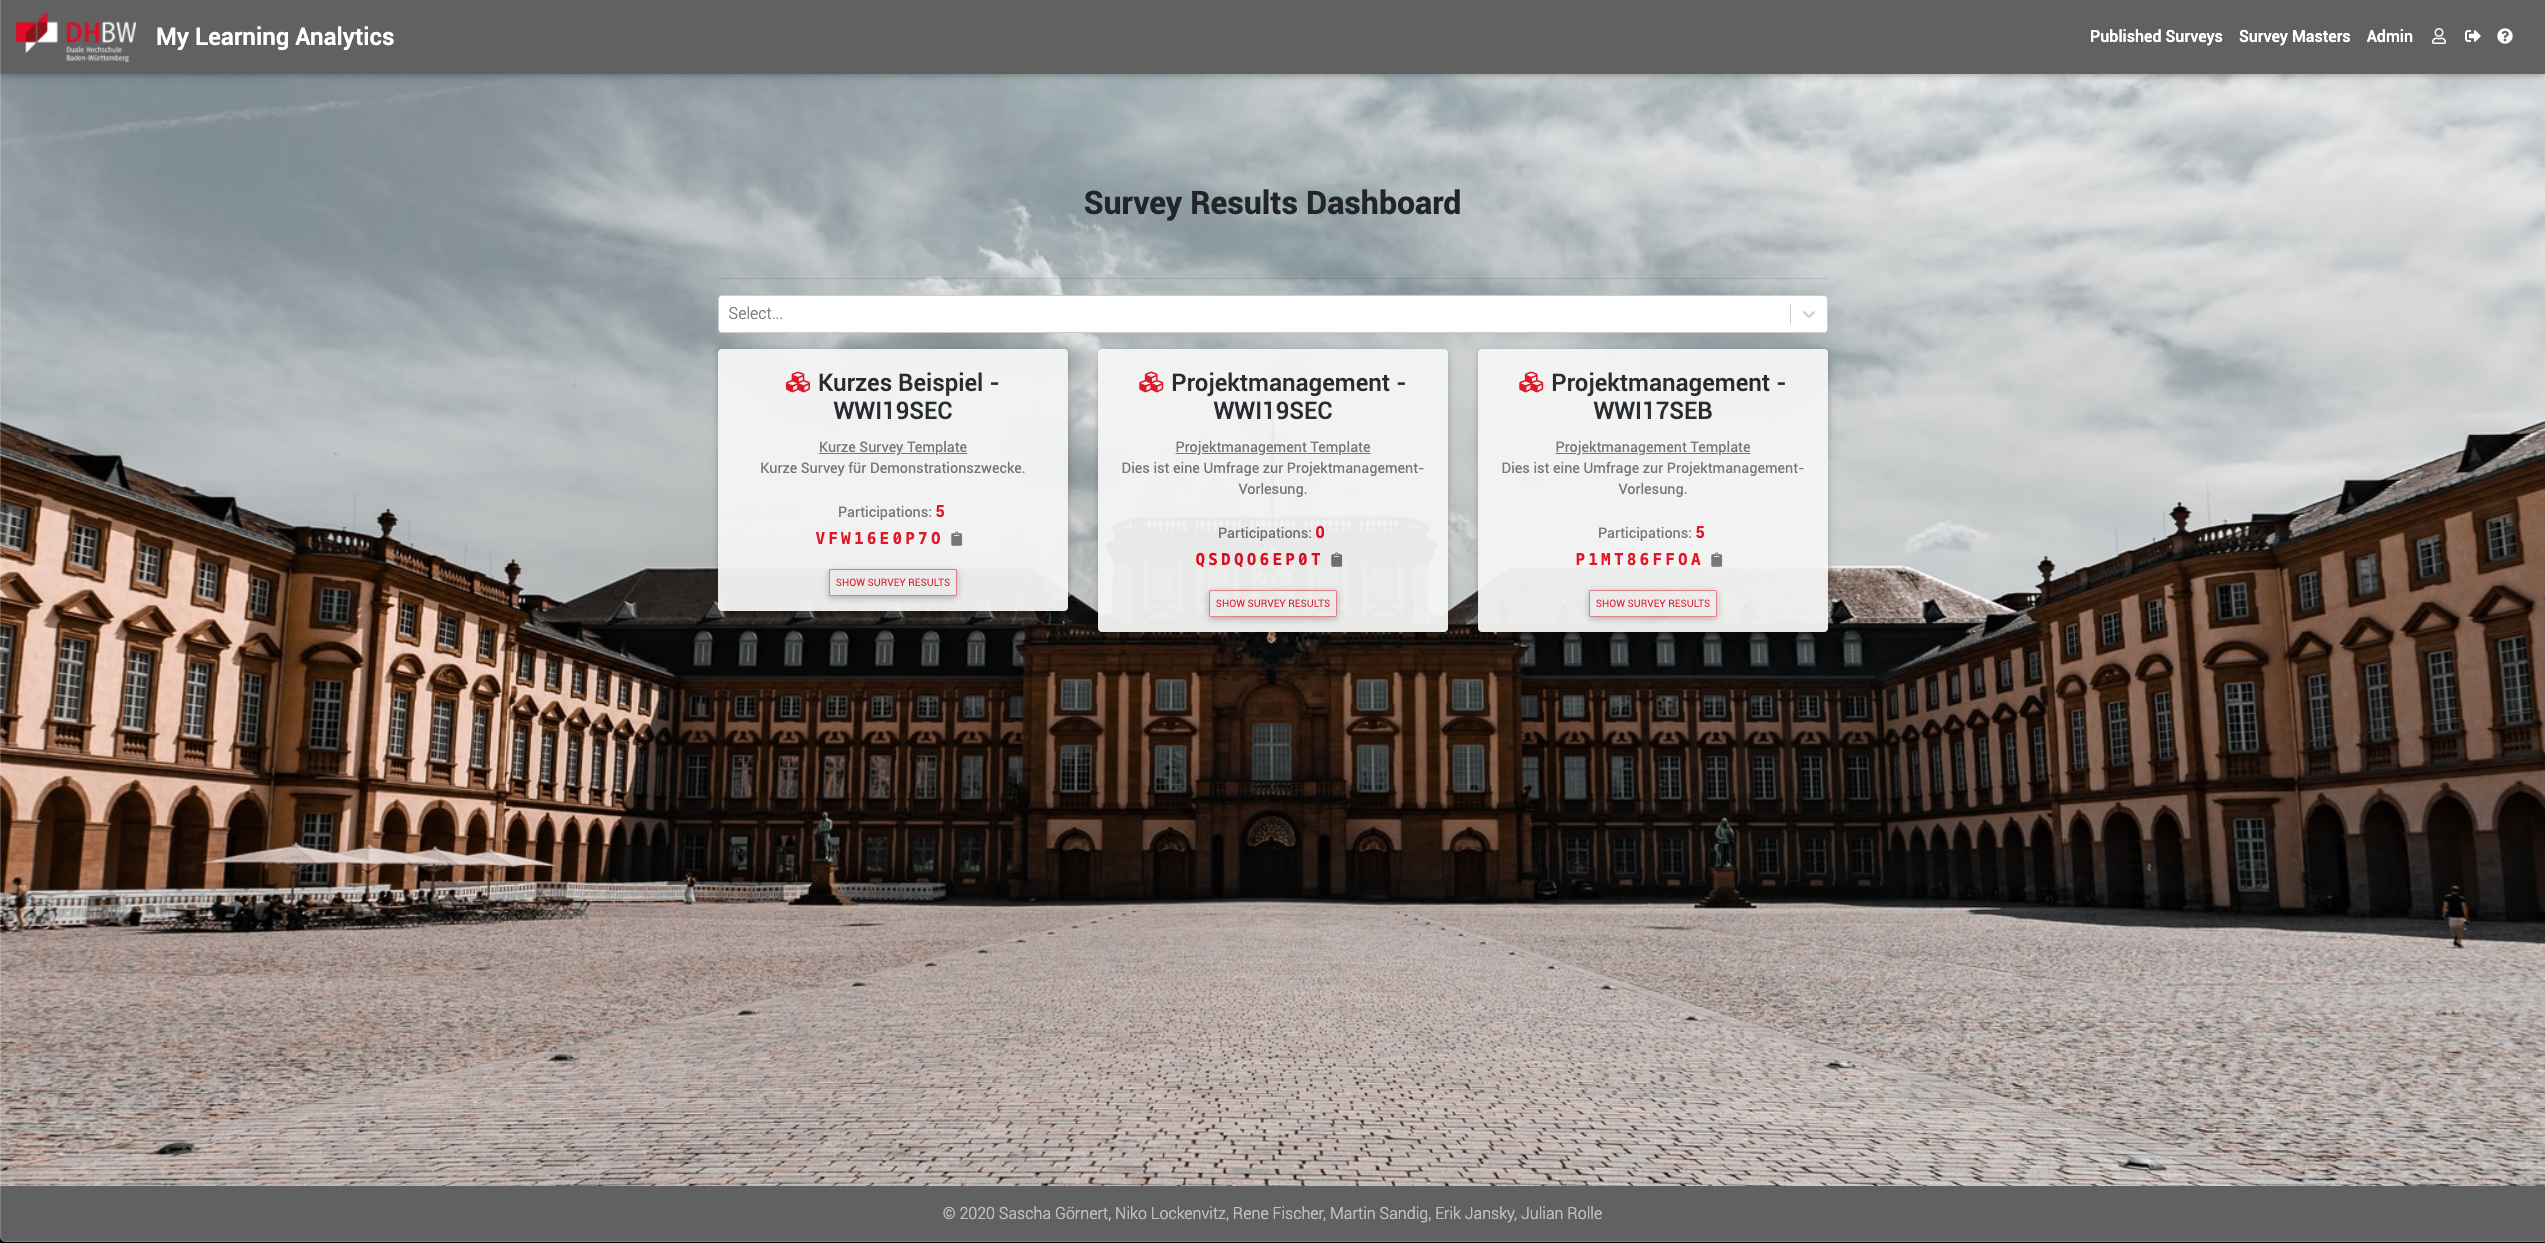
\includegraphics[width=0.95\textwidth, keepaspectratio]{img/client/SurveyResultDashboard.png}
	\captionsetup{justification=centering, format=plain}
	\caption[\acl{UI}: Result-Dashboard]{\acl{UI}: Result-Dashboard \\ \quelleScreenshot}
	\label{fig:SurveyResultDashboardImplement}
\end{figure}

\subsubsection*{Detaillierte Auswertung}
Hat der Benutzer die detaillierte Auswertung ausgewählt, soll je nach Frageart ein bestimmtes Diagramm erstellt werden.
Die Diagramme werden mithilfe von \emph{react-chartjs-2} generiert.\footnote{\url{https://www.npmjs.com/package/react-chartjs-2}}

Abbildung~\myRefGeneral{fig:SurveyResultDetailImplement} zeigt einen Ausschnitt der Auswertung der Umfrage zur Projektmanagement-Vorlesung.
Hier wird exemplarisch ein \emph{Tortendiagramm} ausgegeben.
Die verwendeten Farben wurden zuvor definiert.
Der Benutzer hat die Möglichkeit, seine Maus über das \emph{Tortendiagramm} zu bewegen (hovern).
Hierbei bekommt er den jeweiligen Wert über einen \emph{Tooltip}\footnote{Es öffnet sich ein kleines Fenster, welches Informationen zum ausgewählten Element beinhaltet.} angezeigt.
Dadurch wird Anforderung~\hyperref[Anf:A13]{A13}, die grafische Darstellung der Umfrageergebnisse, erfüllt.

\begin{figure}[!htb]
	\centering
	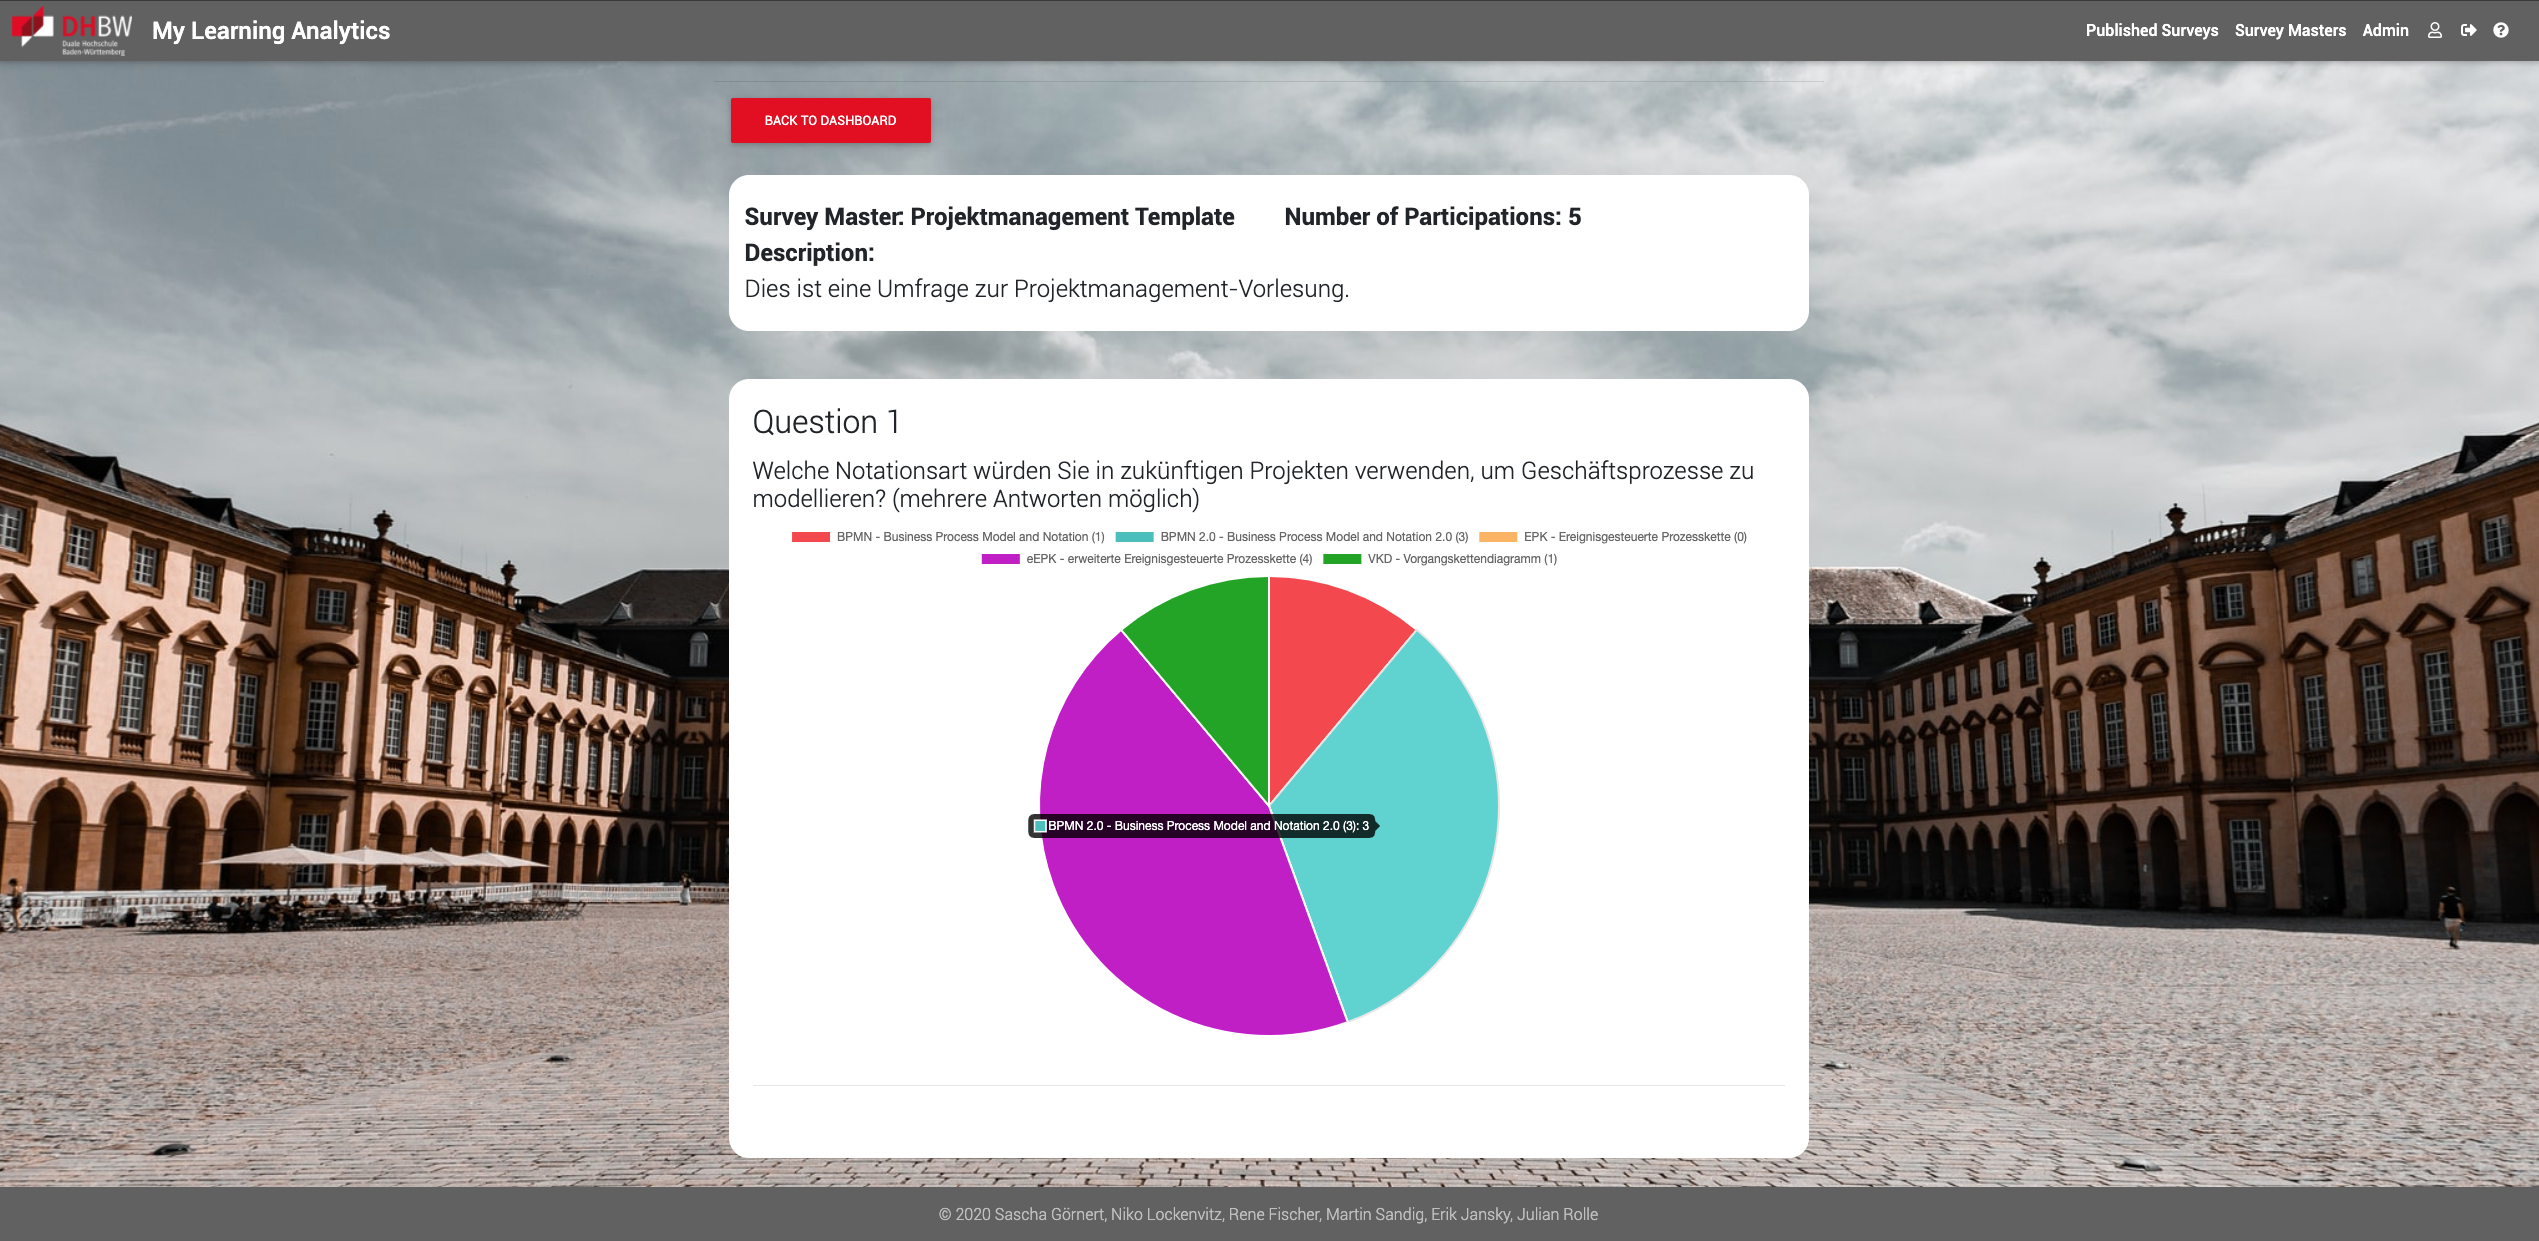
\includegraphics[width=0.95\textwidth, keepaspectratio]{img/client/SurveyResultDetail2.png}
	\captionsetup{justification=centering, format=plain}
	\caption[\acl{UI}: Auswertung der Umfrage]{\acl{UI}: Auswertung der Umfrage aus Abbildung~\vref{fig:SurveyResultDashboardImplement} \\ \quelleScreenshot}
	\label{fig:SurveyResultDetailImplement}
\end{figure}
